
Since our aim is to achieve content-deduplication of the block-cache,
we build an I/O redirection system positioned above the block-cache
which uses implicit caching hints to perform the redirection.
In this section, we first present the requirements of such an I/O redirection 
system and then present our design of the DRIVE (\underline{D}isk I/O
\underline{R}eduction \underline{i}n \underline{V}irtualized 
\underline{E}nvironments\nomenclature{DRIVE:}{\underline{D}isk I/O
\underline{R}eduction \underline{i}n \underline{V}irtualized 
\underline{E}nvironments}) system that meets the specified
requirements\index{DRIVE}.

\subsection{Core idea}
The DRIVE approach dynamically builds metadata based on
similarity identified in disk I/O content by trapping it
upstream from an existing (block-based) disk cache. Using
the metadata information as ``caching hints'', a request
for a disk block is redirected as a request for
another block containing duplicate content, in the hopes
that the requested block has higher likelihood of being
present in cache than the original block. Over time, duplicate
blocks containing identical content will get flushed out
of the cache and the cache will start functioning like a
content-deduplicated cache. Thus, we manipulate an existing
block-based cache like a content-based cache using only
implicit caching hints, without physically changing any
of the caching algorithms or data structures.

\subsection{System requirements}
To perform I/O redirection, metadata needs to be maintained
regarding the similarity of content present in read and write requests. 
Due to inherent content similarity in the workloads,
multiple blocks (i.e. blocks with distinct block ID) have identical content,
and can be represented by a single abstract entity, called a 
a \textit{deduplicated block}. The requirements of an efficient 
I/O reduction system can be stated as follows,
\begin{enumerate}
            \item Fingerprinting mechanism to identify content similarity across
                different blocks.
            \item Data-structures to store metadata for similar blocks.
            \item Maintaining implicit caching hints within metadata to aid
                future I/O redirection.
            \item Interception of block read \textit{request} path for 
                metadata lookup and I/O redirection, if present.
				\index{Interception}
            \item Interception of block read \textit{return} path for
                metdata update, if not previously present.
            \item Interception of block write \textit{request} path for 
                metadata invalidation.
            \item (Optional) Interception of block write \textit{return} 
				path for metadata update.
\end{enumerate}
The above interceptions of block read path may result in longer flow paths,
however, the increased number of cache-hits are expected to outweigh
the effect of increased latencies.
Additionally, the interceptions of block write path should not be too ``costly''
if the underlying cache is in \textit{write-back mode}. However, 
if the cache is in \textit{write-through mode}, the extra latency
due to metadata update may be considerably negligible. 
In the rest of this section, we present the design of the DRIVE system
which addresses all the requirements discussed above.

\subsection{System design}
The DRIVE system has three main components: (i)~Metadata maintenance,
whereby metadata\index{Metadata} 
is maintained to indicate the similarity among blocks being 
accessed in every read and write request, 
(ii)~Maintaining implicit hints regarding host-cache state, wherein the 
blocks which have been recently fetched are noted as \textit{implicit hints} 
that they are more likely to still be in cache when requested next, and
(iii)~Hint-based read I/O redirection, wherein previously stored 
\textit{implicit hints} are used to substitute, if possible, the block 
ID present in the read request with another block ID of duplicate content.
Next, we explain each of these aspects in more detail.

\subsubsection{Metadata maintenance}
%\subsubsection{Design of Metadata store}
The metadata store contains information regarding identical blocks,
where every block is represented by a block ID, and multiple identical
blocks (with distinct block IDs) are mapped to a unique abstract block
of content called a \textit{deduplicated block}\index{Deduplicated block}.
A \textit{deduplicated block} is
associated with, and identified by, a fingerprint of the content.
Thus, each block maps to a unique deduplicated block and every
deduplicated block can potentially reverse map to multiple blocks
in the system. This is depicted in Fig.~\ref{fig:deduped-block}.

\begin{figure}
    \centering
    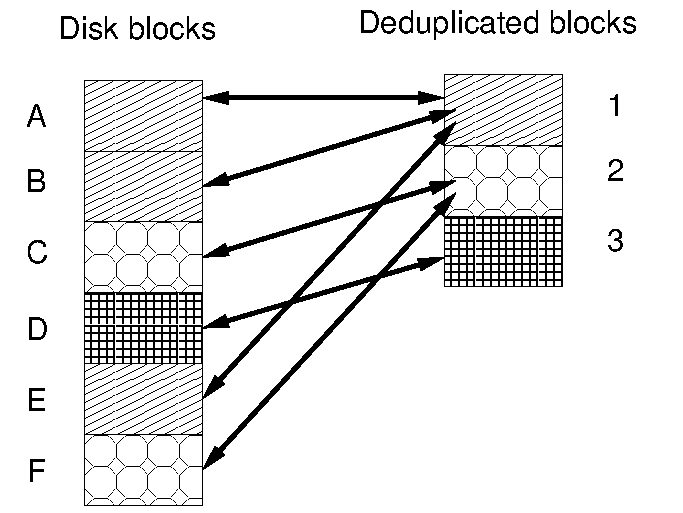
\includegraphics[scale=0.6]{confided-figures/main/deduped-block.pdf}
%    \vspace{-0.15in}
    \caption{Semantics of metadata store in DRIVE system: \textit{each block points to a unique deduplicated block, and each deduplicated block reverse maps to multiple actual blocks}}
    \label{fig:deduped-block}
%    \vspace{-0.2in}
\end{figure}

%\subsubsection{Maintaining metadata}
Metadata can either be built by an \textit{a-priori} scan of the entire
file-system/disk or, at \textit{runtime} as and when read/write
requests are serviced. The advantage of building metadata a-priori is that
when a particular block is requested, its metadata may already be
available,
whereas in case of runtime metadata updates, mapping information for
every block can be known only after the block has been fetched from disk
the first time.
On the other hand, an advantage of runtime metadata updates is that,
metadata needs to be stored only for those blocks that are in the workload,
hence saving space, as compared to an a-priori scan that will build metadata
of the entire disk space. We choose to build metadata at runtime in the
DRIVE system because in most workloads, only a small fraction of the 
entire file-system is actually accessed from the disk~\cite{iodedup}.

Metadata is to be built/updated for every new block of content, to ensure that
it is up-to-date for customized VMs and long-running applications.
In case of read and write requests, block content is encountered in two ways:
(i)~every block of data written to cache for later flushing to disk,
(ii)~every read request for an as yet unseen block (and hence) fetched
from disk. 
In the case of read requests, we compare the 
content fingerprint\index{Content fingerprint}
with existing fingerprints to determine
whether it is ``new'' content or ``duplicate'' of previously seen content,
and update metadata accordingly.
In case of write requests, we invalidate existing mappings for those blocks,
so that stale metadata is not used for the next read request redirection.

\subsubsection{Maintaining hints regarding host-cache state}
When a read request from the front-end driver is serviced by the back-end
driver, it is obvious that the physical block\index{Physical block}
corresponding to the requested
block ID has been recently brought into the host-cache. Thus, if the delivered
content is found to be identical to any other previously requested block, it 
is not only noted 
so in the metadata, but also the most recently fetched block ID is appointed
as the \textit{leader}. This appointment as \textit{leader} is done to aid
redirection of future I/O requests that request the same content, and is
a \textit{hint} regarding the state of host-cache.
Since we do not wish to actively track the host-cache state (i.e., by
trapping and intercepting each insertion and eviction within host-cache), 
these are merely hints and do not guarantee a cache-hit upon I/O redirection.
However, since the hint indicates the most recent block ID with identical
content having been fetched into host-cache, picking that block ID for 
redirection is our best chance of encountering a cache-hit to fetch the 
desired content. 
%The logic of I/O redirection in DRIVE is described next.


%The rationale behind this approach is that
%popular content will translate to popular \textit{leaders}, so if we repeatedly
%pick the leader, we increase its propensity to be in cache when we
%ask for it the next time. Naturally, a cache miss will simply result in a
%disk fetch without incurring any further significant delay. To implement
%this, we use the list of reverse mappings mentioned above. The \textit{head}
%of list is always considered the leader, since it is intuitive
%that the block that was fetched the latest into cache is
%the one that is marked at the head of list of reverse mappings. So,
%picking that block ID as leader is our best chance of
%encountering a cache-hit to fetch the desired content.

\subsubsection{Read I/O redirection using implicit hints}
The DRIVE system uses metadata to achieve non-invasive
cache manipulation by redirection of read I/O requests. Every block read
request is intercepted and metadata looked up to retrieve the corresponding
deduplicated block ID. If the
deduplicated block reverse maps to multiple blocks, it indicates that the 
requested block has identical content as each of the reverse-mapped blocks.
Thus, fetching any of those blocks would suffice to retrieve the content 
being requested, instead of fetching anew from disk. Note that, among the 
reverse mapped blocks, we have flagged the most recently fetched block ID as 
\textit{leader}, as described above. Hence, after interception of the read 
I/O request, we replace the original block ID with the \textit{leader} block ID.

\begin{figure}[t]
    \centering
    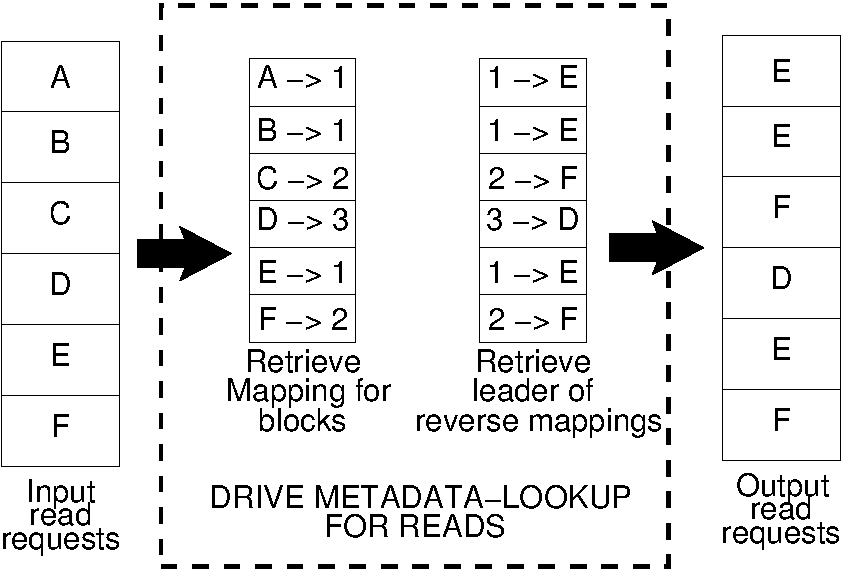
\includegraphics[scale=0.6]{confided-figures/main/dedup-working-reads.pdf}
%    \vspace{-0.125in}
    \caption{Example of read request redirection in DRIVE system}
    \label{fig:confided-working(a)}
%    \vspace{-0.15in}
\end{figure}

A simple example to elaborate on the above redirection approach, is visually
illustrated in Fig.~\ref{fig:confided-working(a)}.
Suppose blocks A, B and E have identical content, and hence 
are mapped to deduplicated ID 1
(refer Fig.~\ref{fig:deduped-block}),
and E is appointed \textit{leader} since it was the most recently fetched
among the three.
Whenever next, read requests for A, B or E are received, redirect the request
to always read block E such that the number of times that block E or its
duplicates are requested, governs the popularity of block E in the cache.
Note that, blocks A, B and C will be in cache the first time that they 
are fetched but once the caching policy eventually evicts them, they
will never enter cache again, unless writes are done to them. This implies
that the cache is operated in an almost fully content-deduplicated fashion,
hence improving its effectiveness in reducing the number of disk reads.

\begin{figure}[t]
    \centering
    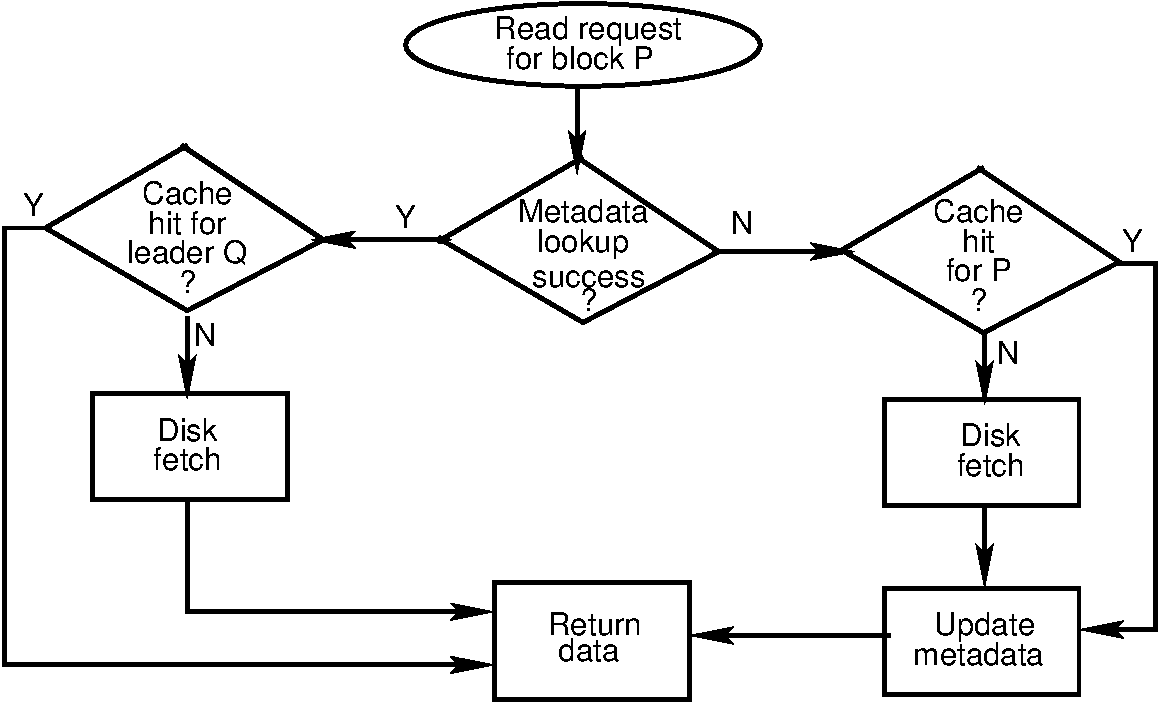
\includegraphics[scale=0.65]{confided-figures/main/dedup-working-readflowcomp.pdf}
    \caption{Flow path(s) for read requests in DRIVE system: \textit{P is the requested block ID and Q is the corresponding ``leader'' block ID.}}
    \label{fig:confided-working(b)}
%     \vspace{-0.25in}
\end{figure}

The above example assumes that all blocks being requested, already
have metadata available. However, in case of
runtime mapping, the first occurrence of every block will result in a
metadata lookup failure and a mandatory disk fetch.
Thus, a read request can have multiple flow paths:
(i)~metadata lookup failure, resulting in fetch from disk,
(ii)~metadata lookup success, but cache miss, resulting in fetch from disk, and
(iii)~metadata lookup success, and cache hit.
If we maintain metadata store also as a limited-size cache, 
%thus foregoing the assumption of infinite metadata space, 
we would encounter two additional flow paths:
(iv)~metadata lookup failure, and cache miss (if previously 
non-leader block), resulting in fetch from disk, and
(v)~metadata lookup failure, and cache hit (if previously leader block).
Fig.~\ref{fig:confided-working(b)} depicts these multiple flows,
wherein an incoming request for block P is looked up in metadata store and if
successful, redirected to block Q. It follows that, Q equals P, \textit{iff}
P is itself the \textit{leader} in the corresponding reverse mappings.
%\\
%\\
%In this section, we described the design of DRIVE system, 
%including the rationale for various design decisions. In the next section, we
%discuss its implementation and associated overheads.

